\chapter{システムの実装方法}
\label{chp:reference}

\section{システム構成}
\label{sec:reference_ftnote}
本システムは以下のような構成で実装を行う.システム構成図を図3.1に示す.\\
労務管理支援システムをReactでWebアプリとして作成した.さらにデータベースにCloud Firestore,
ユーザー認証にFirebase Authentication,表情分析にface-api.jsを使用した。\\
 次のセクションでは,それぞれのサービスについて説明する.

\begin{figure}[!h]
	\begin{center}
			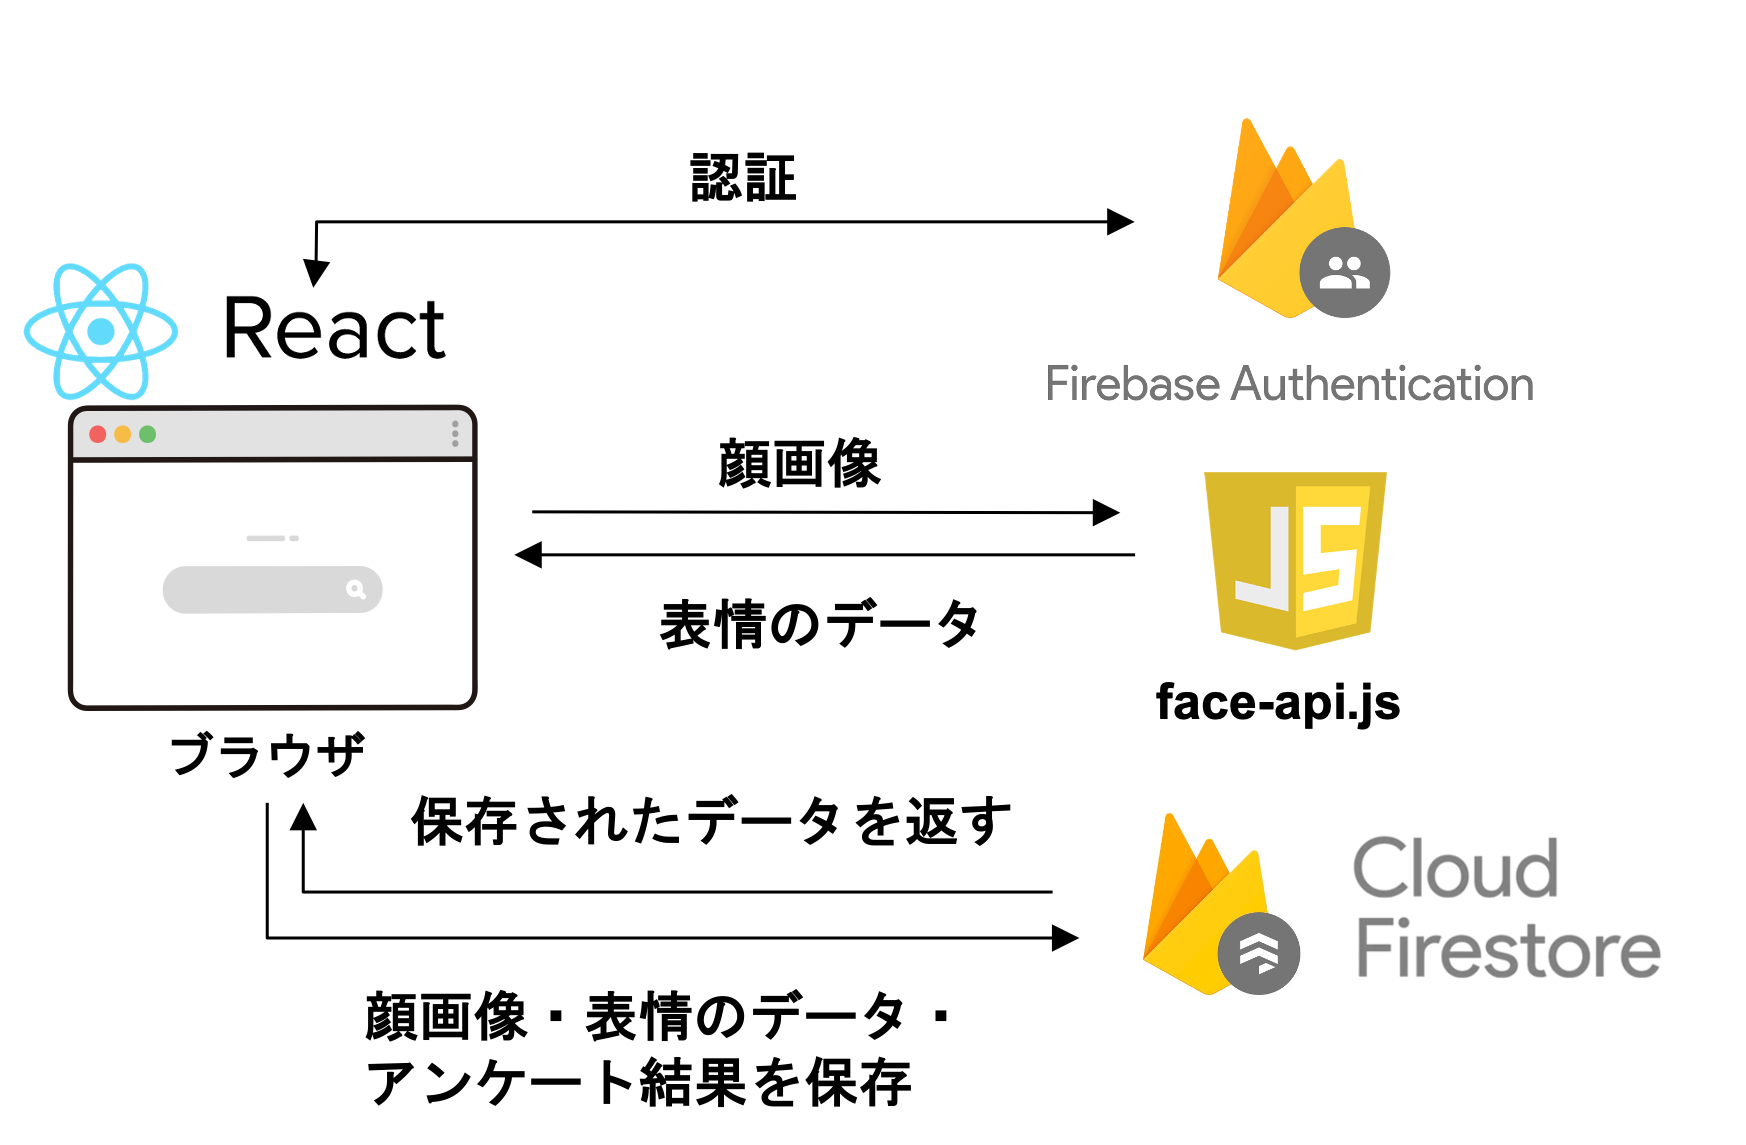
\includegraphics[scale=1.2, clip]{./img/compose.png}
			\caption{システム構成図}
			\label{fig:図の名前}
	\end{center}
\end{figure}


\section{React}
\label{sec:reference_quote}
Reactは,UI(ユーザインタフェース)部分の構築に特化したJavaScriptのライブラリで,
React.jsとも呼ばれる.
SNSで有名なMeta社(旧Facebook社)が自社サービスの機能拡張に伴うコードの複雑化によって
維持管理がしにくくなることを防ぐために開発した.
コーディングコストが少なく,開発規模が大きくなっても管理しやすいといった特長もあり,
現在では開発元であるFacebook社のサービスであるFacebookやInstagramはもちろんのこと,
Yahoo!やAirbnb,Reddit,Netflix,Slack,Uberといった世界的なWebサイトや
Webアプリで利用されるなど,世界中の多くの企業で採用されており,日本でも注目を集める
など,今最も勢いのあるライブラリである.
今回のシステム開発にReactを採用した理由は三つある.

	\begin{enumerate}
		\item パフォーマンスが良い \\
		Reactには,仮想DOM(Virtual Document Object Model)というレンダリング機構が
		備わっている.仮装DOMとは、実際のDOMではなく, React内部に持っている 
		DOMの情報である. Reactを使うと,この仮想DOMと実際のHTML上のDOMを
		比較したときに出てくる違いだけが,毎回HTML上に再適用される.
		そのため画面全体がReactで構成されていたとしても,必要な部分しか更新されず
		非常に高速に動作するため,パフォーマンスが良い.\\

		\item UIコンポーネントのライブラリが多い \\
		Reactは,世界中で使われているため,Reactのライブラリを使ってUIをコンポート化
		するようになってきている.あらかじめButtonやFormなどのUIパーツを
		Reactコンポーネントとして扱えるようにして,セット化したものが多くある.
		これらを使えば,今風の洗練された画面を作ることができる.\\

		\item JavaScriptの知識があれば使える \\
		基本的にReactはJavaScriptで書かれているため,
		JavaScriptの知識があればアプリを開発することができる.
		たとえJavaScriptの開発経験がなくても基本構文を理解していれば開発に
		取り掛かれる.今回,我々はJavaScriptの学習を既に行なっていたので,
		Reactを選んだ.
	\end{enumerate}
	
\section{face-api.jsについて}
\label{sec:reference_bib}
face-api.jsはブラウザ, NodeJSで顔を検出するための,
Tensorflow.jsを活用したJavaScript APIである.
ここでは,face-api.jsがどのような機能を提供しているかを紹介する.
\begin{itemize}
	\item 顔検出 \\
	写真から顔を探して検出する. \\

	\item 顔のランドマーク検出 \\
	検出した顔の目や鼻の位置など,顔の特徴を抽出する上で重要なキーポイントを検出する. \\

	\item 表情認識 \\
	検出した顔の表情を認識する.表情は,「怒り」,「嬉しさ」,「中立」,「恐怖」,「うんざり」,
	「驚き」,「悲しさ」の7種類あり,数値で表される. \\

	\item 年齢推定 \\
	検出した顔の年齢を推定する. \\

	\item 性別認識 \\
	検出した顔の性別を推定する. \\

	今回は,顔検出と表情認識の機能を使い,表情分析した値をグラフ化することを目的とする.
\end{itemize}
	
\section{Material-UIについて}
\label{sec:reference_chapter}

